\newpage

\begin{justify}
    Στο 3\textsuperscript{ο} και τελευταίο ερώτημα, θα προσομοιωθεί
    ένα \textlatin{PAM} σύστμα βασικής ζώνης, το οποίο μεταφέρει
    $N$ \textlatin{bits} χρησιμοποιώντας διαμόρφωση \textlatin{2-PAM}.
    Για $T=10^{-2}$\textlatin{sec}, \textlatin{over}$=10$, $α=0.5$,
    και $Α=4$. (το $Α$ ισούται με το μισό μήκος του αποκομμένου 
    παλμού μετρημένο σε περιόδους συμβόλου).\\\\
    {\bf \textlatin{C.1}} (5) Να δημιοργήσετε $N$ \textlatin{bits}
    $b\textsubscript{i}$ για $i=0,1,..N-1$ ($N=50,100$), με την
    εντολή $b=(sign(rand(N,1))+1)/2$:\\\\
    \textbf{Λύση:}
\end{justify}

\vspace{-2em}
    
%%%%%%%%MATLAB code
\textlatin{
    \lstinputlisting[language=Matlab,]{CE/Matlab/C1.m}
} 

\begin{justify}
    {\bf \textlatin{C.2}} Το σύστημα \textlatin{2-PAM} υλοποιείται
    ως εξής.\\\\
    {\bf (α)} (5) Να γράψετε την συνάρτηση
    $X=bits\_to\_2PAM(b)$ η οποία παίρνει είσοδο την ακολουθία
    \textlatin{bits b} και παράγει ως έξοδο την ακολουθία από
    \textlatin{2-PAM} σύμβολα $X$, χρησιμοποιώντας την εξής απεικόνιση:
    \[ 0 \rightarrow +1, \]
    \[ 1 \rightarrow -1. \]
\end{justify}

\begin{justify}
    \textbf{Λύση:}\\
    Η συνάρτηση επιστρέφει $X=-1$ με είσοδο $b=1$ και 
    $X=1$ όταν $b=0$.

\end{justify}

\vspace{-2em}

%%%%%%%%MATLAB code
\textlatin{
    \lstinputlisting[language=Matlab,]{CE/Matlab/C2A.m}
} 

\newpage

\begin{justify}
    {\bf (β)} Να προσομοιώσετε το σήμα:
\end{justify}

\[
    X_{\delta}(t)=\sum_{k=0}^{N-1}X_{k}\delta(t-kT)
\]

\begin{justify}
μέσω της εντολής:
\end{justify}
\[
    X\_delta=1/Ts*upsample(X,over).
\]

\begin{justify}
    (10) Να ορίσετε κατάλληλα τον άξονα του χρόνου και να σχεδιάσετε
    το σήμα $X_{\delta}(t)$.\\\\
    \textbf{Λύση:}
\end{justify}
    
\vspace{-2em}

%%%%%%%%MATLAB code
\textlatin{
    \lstinputlisting[language=Matlab,]{CE/Matlab/C2B.m}
} 

\newpage

\begin{justify}
    Όπως βλέπουμε σχεδιάσαμε ένα τρένο παλμών κλιμακομένο κατά 
    $1/T_{s}$.
\end{justify}

%%%%%%PLOT
\begin{center}
    \centering
    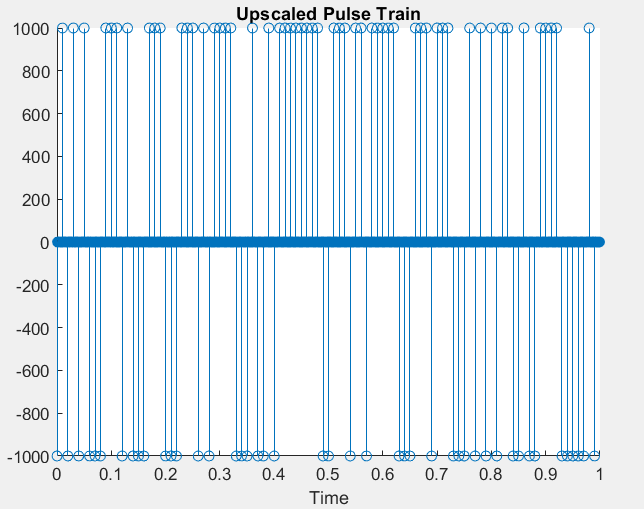
\includegraphics[width=0.8\textwidth]{CE/Images/c.1.png} % Adjust width as neededfilename of your images
\end{center}



\begin{justify} 
    {\bf (ς)} Να δημιουργήσετε αποκομμένο \textlatin{SRRC}
    παλμός $\phi(t)$(χρησιμοποιώντας τις παραπάνω παραμέτρους) και 
    να προσομοιώσετε την συνέλιξη $X(t)=X_{\delta}*\phi(t)$.\\\\
    (10) Να κατασκευάσετε κατάλληλα τον άξονα
    του χρόνου και να σχεδιάσετε το σήμα $X(t)$.\\\\
\end{justify}

\vspace{-2em}

%%%%%%%%MATLAB code
\textlatin{
    \lstinputlisting[language=Matlab,]{CE/Matlab/C3.m}
} 

\newpage

%%%%%%PLOT
\begin{center}
    \centering
    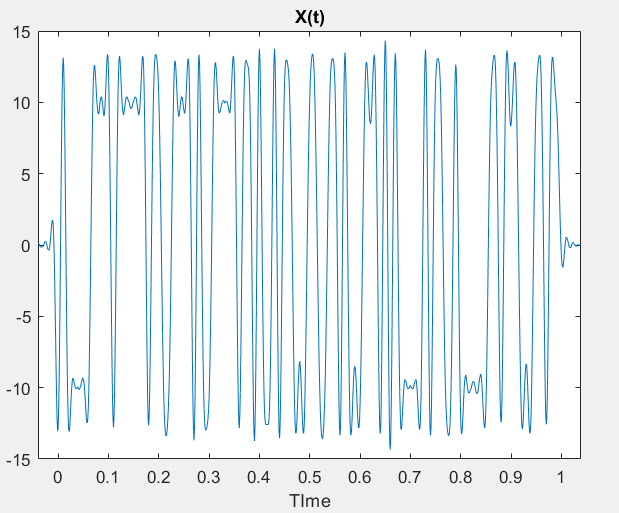
\includegraphics[width=0.8\textwidth]{CE/Images/c.2.png} % Adjust width as neededfilename of your images
\end{center}

\vspace{1.5em}

\begin{justify}
    {\bf (δ)} Υποθέτοντας ιδανικό κανάλι, στην είσοδο του δέκτη
    λαμβάνουμε $X(t)$. Να προσομοιώσετε τη συνέλιξη $Z(t)=X(t)*\phi(-t)$.\\\\
    (10) Να σχεδιάσετε το $Z(t)$ στον αντίστοιχο άξονα του χρόνου
    και να βρείτε τι τιμές παίρνει τις χρονικές στιγμές $kT$, για
    $k=0,...,N-1$.Μπορείτε να εξηγήσετε το φαινόμενο\textlatin{;}\\\\
    \textbf{Λύση:}\\
    Χρησιμοποιήθηκε ο ίδιος αποκομμένος \textlatin{SRRC} παλμός
    διότι είναι άρτια συνάρτηση ($\phi(t)=\phi(-t)$).
\end{justify}

\vspace{-2em}

%%%%%%%%MATLAB code
\textlatin{
    \lstinputlisting[language=Matlab,]{CE/Matlab/C4.1.m}
} 

%%%%%%PLOT
\begin{center}
    \centering
    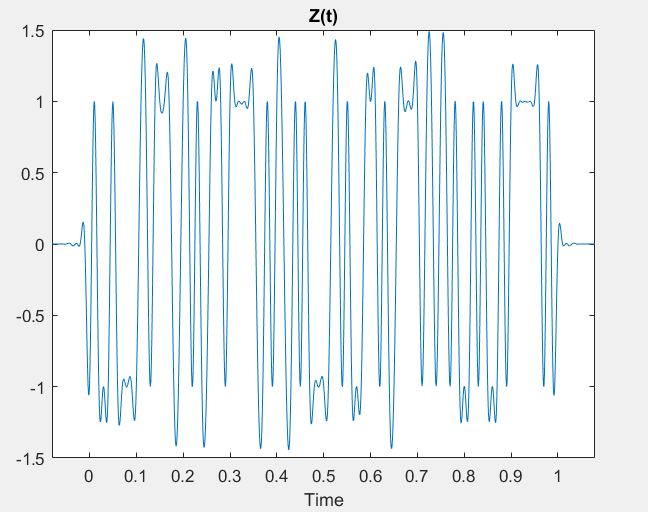
\includegraphics[width=0.8\textwidth]{CE/Images/c.3.png} % Adjust width as neededfilename of your images
\end{center}

\begin{justify}
    (5) Ένας γραφικός τρόπος για να συγκρίνεται τις τιμές
    $Z(kT)$ με τις τιμές $X_{k}$, για  $k=0,...,N-1$, είναι να
    επιλέξετε \textlatin{hold on} στο \textlatin{plot} του
    $Z(t)$ και να εκτελέσετε την εντολή \textlatin{stem([0:N-1]*T,X);}
    όπου $Χ$ είναι το διάνυσμα με τα σύμβολα $X_{k}$, $k=0,...,N-1$.\\\\
    \textbf{Λύση:}\\
\end{justify}

\begin{justify}
    Βρίσκουμε τις θέσεις του $Z(t)$ που μας ενδοιαφέρουν
    δηλαδή από την χρονική στιγμή $t=0$ ως την χρομνική στιγμή
    που τελειώνει το τρένο παλμών. Έχοντας τον παλμό που μας ενδοιαφέρει
    \textlatin{zsampled} τον κάνουμε \textlatin{downsample}.\\\\
    Ακολουθεί ο κώδικας \textlatin{Matlab}: 
\end{justify}

\vspace{-2em}

%%%%%%%%MATLAB code
\textlatin{
    \lstinputlisting[language=Matlab,]{CE/Matlab/C4.2.m}
} 

%%%%%%PLOT
\begin{center}
    \centering
    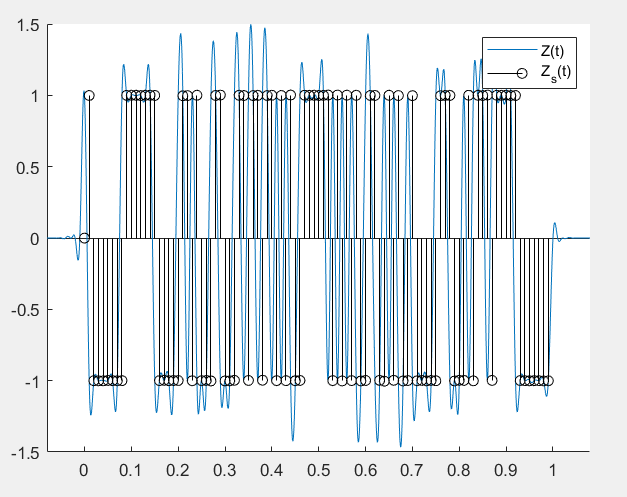
\includegraphics[width=0.8\textwidth]{CE/Images/c.4.png} % Adjust width as neededfilename of your images
\end{center}




